\subsection{Описание структуры приложения}
\label{sec:development:app_structure}

На рисунке~\ref{sec:development:app_structure_pic} представлена файловая структура проекта, который является клиентским приложением.

\begin{figure}[ht]
\centering
    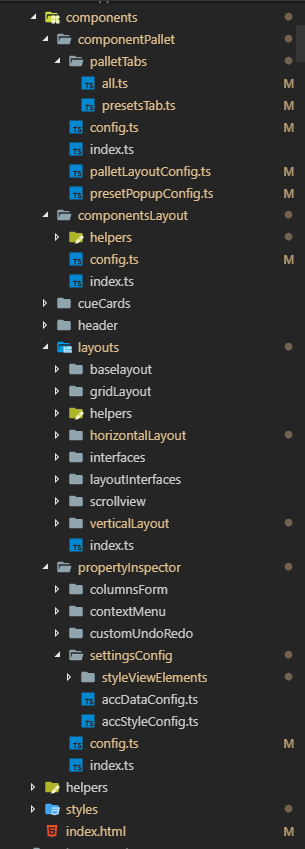
\includegraphics[scale=0.6]{dev_app_structure.png}
    \caption{Файловая структура проекта}
    \label{sec:development:app_structure_pic}
\end{figure}

Проект состоит из следующих основных частей:

\begin{itemize}
    \item папка Components, содержащая исходный код компонентов;
    \item папка helpers, содержащая некторые часто применяемые участки кода, вынесенные в отдельные функции;
    \item папка styles, содержащая CSS-стили для всего проекта.
\end{itemize}

Папка Components в свою очередь включает в себя все существующие компоненты и состоит из:

\begin{itemize}
    \item папка componentsPallet, содержащая исходный код палитры компонентов;
    \item папка componentsLayout, содержащая исходный код грида;
    \item папка cueCards, содержащая исходный код пользовательских шаблонов;
    \item папка layouts, содержащая исходный код основных предоставляемых компонентов;
    \item папка propertyInspector, содержащая исходный код инспектора свойств.
\end{itemize}

Папка layouts, как уже было сказано выше, включает в себя папки, содержащие исходный код каждого из присутствующих в программном компонентов. Этими папками являются:

\begin{itemize}
    \item папка baselayout содержит исходный базового компонента, чья функциональность используется во всех компоненах типа <<layout>>;
    \item папка gridlayout, содержит исходный особого компонента типа <<layout>>, который использует совершенно другой способ позиционироваия дочерних элементов, нежели baselayout: в отличие от последнего, где используется смещение в пикселях от левой верхней точки, здесь используется абсолютное позиционирование по виртуальным клеткам;
    \item папка helpers, содержащая некторые часто применяемые в компонентах участки кода, вынесенные в отдельные функции;
    \item папки horizontal layout и vertical layout содержат исходный код одноименных компонентов, осуществояющих позиционирование дочерних компонентов либо в колонки (горизонтально), либо в строки (вертикально).
\end{itemize}

    